%\section*{Supplementary material of \textit{Mixed-Membership Stochastic Block Models for Weighted Networks}}

\section{Derivation of the collapsed variational updates for WMMSB-bg}
\label{app:collap}

%%%%%%%
%\vspace{0.7cm}
%\section*{Beta-Gamma updates}
%\vspace{0.1cm}
%%%%%%%

In the WMMSB-bg model, the collapsed variational distribution takes the form:

\begin{equation*}
q(\Pi) = q(\Theta, \Phi|Z, R, P) q(Z)q(R)q(P)
\end{equation*}

The variational distribution for $r_{kk'}$ is taken in the Gamma family:  $q(r_{kk'}) = \textrm{Gamma}(a_{kk'},b_{kk'})$ for $1\leq k,k' \leq K$. The collapsed ELBO can thus be rewritten as:
%
\[
\log p(Y) \geq \L_{Z,R,P},
\]
%
with:
\begin{align*}
\L_{Z,R,P} &= \E_{q}[\log p(Y, Z, R, P|\Omega)] + \textrm{H}[q(Z)] \\
& \qquad + \textrm{H}[q(R)] + \textrm{H}[q(P)] \\
& = \E_{q}[\log p(Y, Z)] + \textrm{H}[q(Z)] \\
& \qquad + \E_{q}[\log p(R|Y,Z,P)] + \textrm{H}[q(R)] \\
& \qquad +\E_{q}[\log p(P|Y,Z)] + \textrm{H}[q(P)].
\end{align*}

\paragraph{Optimizing $\gamma_{ijkk'}$}

In the Beta-Gamma augmentation, the parameters $p$ and $r$ are marginalized in the update given by:
%
\begin{align*}
&\gamma_{ijkk'} \propto \nonumber\\
&e^{E_{q(Z^{-ij})} [\log E_{q(r_{kk'})}[E_{q(p_{kk'})}[ P(z_{i\rightarrow j}=k, z_{i\leftarrow j}=k' | Y^{-ij}, Z^{-ij}, \Omega) ] ] ]}
\end{align*}
%
By using a first order Taylor expansion, one obtains:
%
\begin{align*}
\gamma_{ijkk'} & \propto (N_{\rightarrow ik}^{\Theta^{-j}} + \alpha_k) (N_{\leftarrow jk'}^{\Theta^{-i}} + \alpha_{k'}) \\
& \mathrm{NB}\left(y_{ij}; N^{Y^{-ij}}_{kk'} + \E_{q}[r_{kk'}], p' \right),
\end{align*}
%
with:
%
\[
p' = \frac{\E_{q}[p_{kk'}]}{\E_{q}[p_{kk'}]\,N^{\Phi^{-ij}}_{\bm{.}kk'} + 1}.
\]

\paragraph{Optimizing $p_{kk'}$}

In oder to maximize the collapsed ELBO w.r.t $p_{kk'}$, one can let $q(p_{kk'}) = p(p_{kk'} | Y,Z) = E_q(r_{kk'}) [ p(p_{kk'} | Y^{(kk')},Z^{(kk')} ,r_{kk'})]$. As the negative binomial and Beta distributions are conjugate, a closed-form expression can be obtained:

\begin{align*}
& p(p_{kk'} | Y^{(kk')}, Z^{(kk')}, r_{kk'}) \propto p(Y^{(kk')| Z^{(kk')}, r_{kk'}} p(r_{kk'}) \\
& \propto (1-p_{kk'})^{r_{kk'} N^\Phi_{kk'}}p_{kk'}^{N^Y_{kk'}} p_{kk'}^{c\epsilon -1} (1-p_{kk'})^{c(1-\epsilon) -1} \\
& \propto p_{kk'}^{c\epsilon + N^Y_{kk'} -1} (1-p_{kk'})^{c(1-\epsilon) + N^\Phi_{kk'}r_{kk'}-1} \\
& = \mathrm{Beta}(c\epsilon + N^Y_{kk'}, c(1-\epsilon) + N^\Phi_{kk'}r_{kk'}).
\end{align*}

Finally, by resorting again to a first order Taylor expansion, one obtains:
%
\begin{equation*}
p_{kk'} \sim \mathrm{Beta}(c\epsilon + N^Y_{kk'}, c(1-\epsilon) + N^\Phi_{kk'} E_q[r_{kk'}]), \nonumber
\end{equation*}
%
so that:
%
\[
\E_{q}[p_{kk'}] = \frac{c\epsilon + N^Y_{kk'}}{c\epsilon + N^Y_{kk'} + c(1-\epsilon) + N^\Phi_{kk'}\E_{q}[r_{kk'}]}.
\]
%

\paragraph{Optimizing $r_{kk'}$}

To isolate the contribution, in the collapsed ELBO, that depends on $r_{kk'}$ (through $a_{kk'}$ and $b_{kk'}$), we only consider the links that have been generated within the classes $k,k'$, denoted by $Y^{(kk')}$. As $y_{ij} \sim NB(r_{kk'}, p_{kk'})$ if $i$ is in class $k$ and $j$ in class $k'$, one has:

\begin{align*}
\L_{[r_{kk'}]} = & \E_{q(r_{kk'})}[\log p(r_{kk'}|Y^{(kk')},Z^{(kk')},p_{kk'})] \\
& + \textrm{H}[q(r_{kk'})].
\end{align*}

By applying Bayes rules and dropping the normalizing term that does not depend on $r_{kk'}$, one gets:

\small{
\begin{align*}
\L_{[r_{kk'}]} &= \E_{q(r_{kk'})}[\log \left( p(Y^{(kk')}|Z^{(kk')}, r_{kk'}, p_{kk'}) p(r_{kk'}]) \right)] \\
	& \qquad + \textrm{H}[q(r_{kk'})] \\
    &= \E_{q(r_{kk'})}[\log \left( \prod_{ij\in Y^{(kk')}} \dbinom{r_{kk'} + y_{ij}-1}{y_{ij}} \right. \\
    & \qquad  \left. (1-p_{kk'})^{r_{kk'}} p_k^{y_{ij}} p(r_{kk'}) \right) ] + \textrm{H}[q(r_{kk'})] \\
    &= \E_{q(r_{kk'})}[\log \left( (1-p_{kk'})^{r_{kk'} N^{\Phi}_{kk'}} p_{kk'}^{N^{Y}_{kk'}} p(r_{kk'}) \right. \\
    &  \qquad  \left. \prod_{ij\in Y^{(kk')}} \frac{\Gamma(r_{kk'}+y_{ij})}{\Gamma(r_{kk'}) \Gamma(y_{ij}+1) }  \right) ] + \textrm{H}[q(r_{kk'})].
\end{align*}
}

\normalsize

If $y_{ij} = 0$, then $\frac{\Gamma(r_{kk'}+y_{ij})}{\Gamma(r_{kk'}) \Gamma(y_{ij}+1)} = 1$, whereas if $y_{ij} \ne 0$, then $\frac{\Gamma(r_{kk'}+y_{ij})}{\Gamma(r_{kk'}) \Gamma(y_{ij}+1)} = \frac{1}{B(r_{kk'}, y_{ij})y_{ij}}$. Furthermore, in this latter case:
%
\begin{align*}
%B(r_{kk'}, y_{ij}) = \int_0^1 t^{r_{kk'}-1} (1-t)^{y_{ij}-1} dt  \leq \int_0^1 t^{r_{kk'}-1} dt = \frac{1}{r_k}
B(r_{kk'}, y_{ij}) = \int_0^1 t^{r_{kk'}-1} (1-t)^{y_{ij}-1} dt  \leq \frac{1}{r_k},
\end{align*}
%
so that:
%
\begin{equation*}
\log \prod_{ij\in Y^{(kk')}} \frac{\Gamma(r_{kk'}+y_{ij})}{\Gamma(r_{kk'}) \Gamma(y_{ij}+1) } \geq N^Y_{kk'} \log(r_{kk'}) + \mathrm{cst},
\end{equation*}
%
with $N^Y_{kk'} = \sum_{ij\in Y^{(kk')}} y_{ij}$.

Furthermore, from the model definitions, one has: $\log p(r_{kk'}) = (r_0 c_0-1)\log(r_{kk'}) - r_{kk'} c_0 + \mathrm{cst}$  and $\textrm{H}[q(r_{kk'})] = a_{kk'} + \log(b_{kk'}) +\log \Gamma(a_{kk'}) + (1-a_{kk'})\Psi(a_{kk'})$.

Hence:
%
\begin{align*}
\L_{[r_{kk'}]} \geq & N^\Phi_{kk'} a_{kk'} b_{kk'} \log(1-p_{kk'}) \\
& + (r_0 c_0-1 )(\Psi(a_{kk'}) + \log(b_{kk'})) \\
& - c_0 a_{kk'} b_{kk'} + N^Y_{kk'} (\Psi(a_{kk'}) \\
& + \log(b_{kk'}))  a_{kk'} + \log(b_{kk'}) \\
& + \log \Gamma(a_{kk'}) + (1-a_{kk'})\Psi(a_{kk'}).
\end{align*}

Maximizing the right-hand term of the above inequality with respect to $b_{kk'}$ yields:

\begin{equation} \label{eq:update2}
b_{kk'} = \frac{r_0 c_0 + N^Y_{kk'}}{a_{kk'} (c_0 - N^\Phi_{kk'} \log(1-p_{kk'}))}. \nonumber
\end{equation}

As $r_{kk'} \sim \textrm{Gamma}(a_{kk'},b_{kk'})$, one finally obtains:

\begin{equation}
\E_q[r_{kk'}] = a_{kk'} b_{kk'} = \frac{r_0 c_0 + N^Y_{kk'}}{c_0 - N^\Phi_{kk'} \log(1-p_{kk'})}. \nonumber
\end{equation}


%\section{Stratified Sampling}
%
%Sampling from minibatches in SVI, for MMSB model, was initially proposed in [6] and [7]. The adaptation of the sampling scheme for SCVI is based on the reformulation of the "sufficient statistics" $N^\Theta, N^\Phi$ and $N^Y$  by bringing up a minibatch distribution $h(S)$. The idea of the stratified sampling is to divide the edges into subset that share some statistical strength.
%For each node $n$ with divide it's neighbors pairs into a set $S_1$ containing all its links (edges) and a subset $S_0$ dividing into  $m$ set containing its non-links. Then sampling consists of drawing one of its its set $S_0$ or $S_0$ with probability.
%
%\begin{align*}
%h(S)=\begin{cases}
%    \frac{1}{2 N}  & \textrm{ if } S = S_1 \\
%    \frac{1}{2 N m}  & \textrm{ if } S \in S_0 
%    \end{cases}
%\end{align*}
%
%
%By referencing any of the global "sufficient statistics" of the models with the term $N^*$ such that $N^* \in \{N^Y, N^\Theta, N^\Phi\}$. Assuming that every pair (i, j) occurs in some constant number of sets c, $N^*$ can be reformulated as follows 
%
%\begin{align*}
%N^* = \sum_{ij, *} \gamma_{ij} = \E_h[ \frac{1}{c}\frac{1}{h(S)} \sum_{ij \in S, *} \gamma_{ij}  ]
%\end{align*}
%
%Where $N^*$ and $\gamma_{ij}$ are matricies of size $K\times K$.
%The exact summing formulation of $N^*=\sum_{ij,*}$ is given in section 3.1. For undirected network, $c$ is equal to 2 because each pair occurs in two set, and $c$ is 1 for directed network.

\section{Impact of the number of classes}
\label{app:K}

\begin{figure}[ht]
\centering
	
\begin{subfigure}
     \centering
         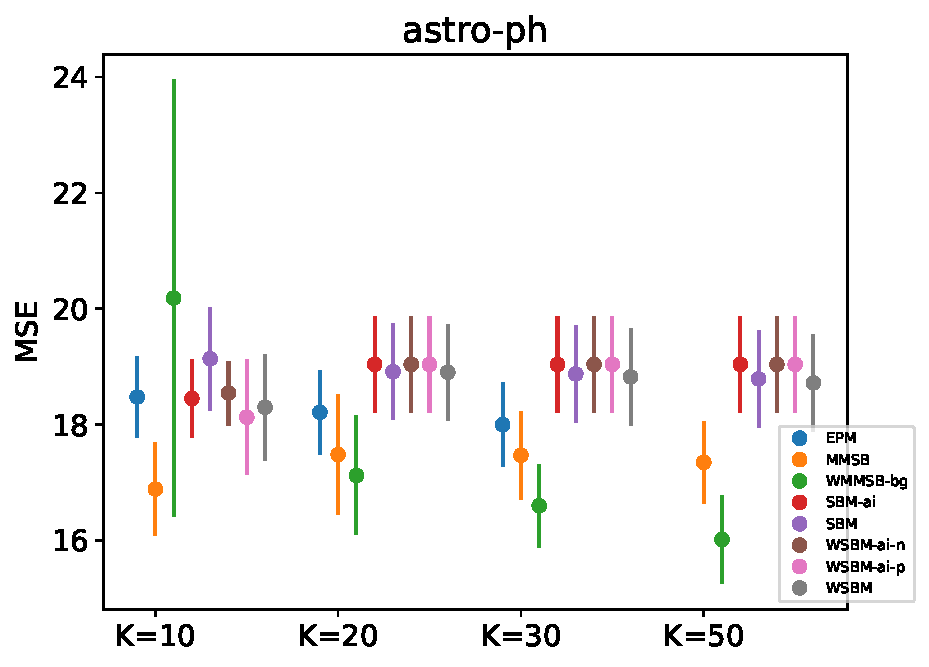
\includegraphics[width=0.23\textwidth]{fig2/astro-ph_wsim3_evo2__}
\end{subfigure}
\begin{subfigure}
         \centering
      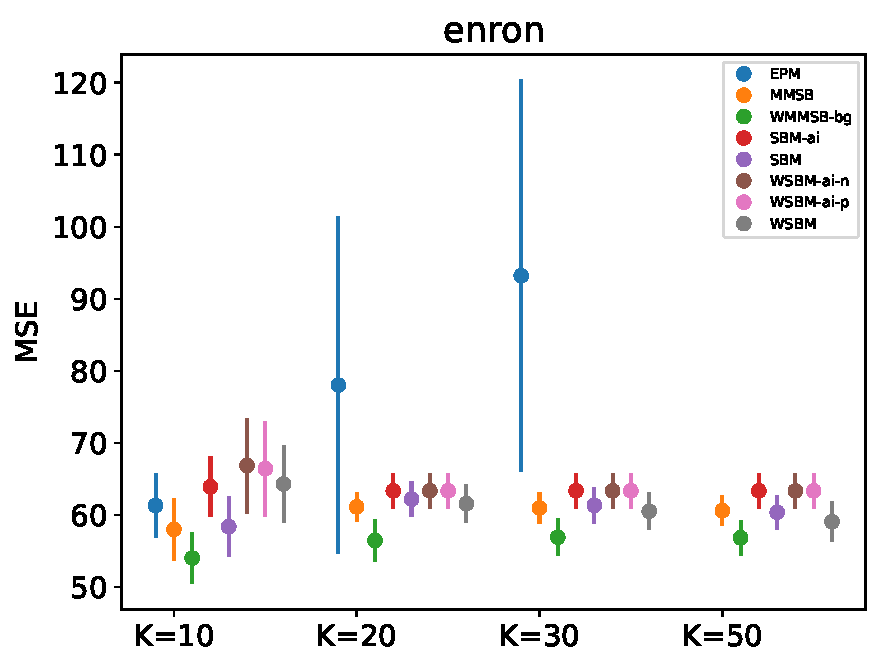
\includegraphics[width=0.23\textwidth]{fig2/enron_wsim3_evo2__}   
\end{subfigure}  
\begin{subfigure}
         \centering          
      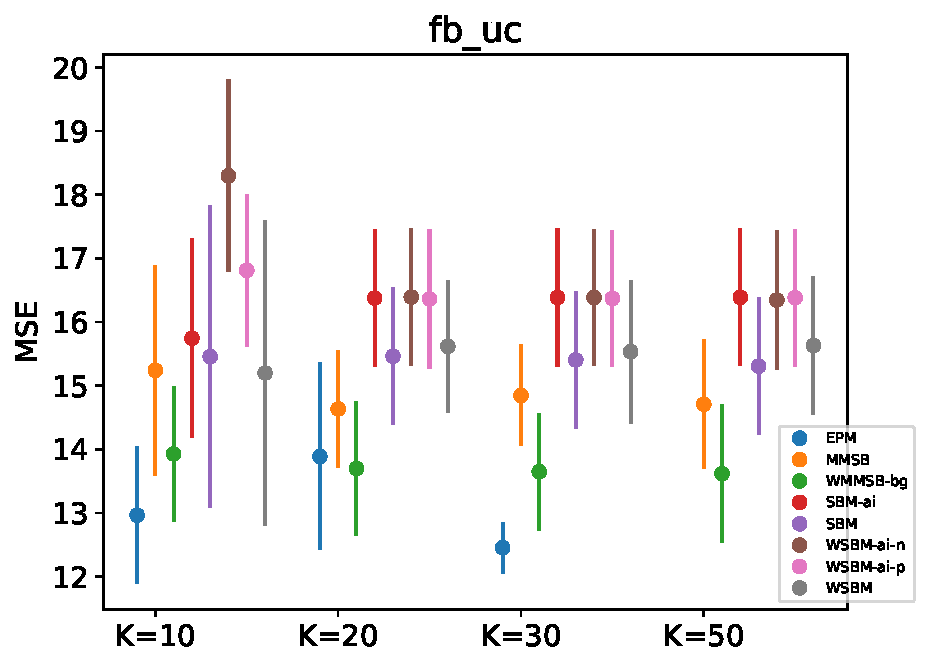
\includegraphics[width=0.23\textwidth]{fig2/fb_uc_wsim3_evo2__}
\end{subfigure}  
\begin{subfigure}
         \centering          
      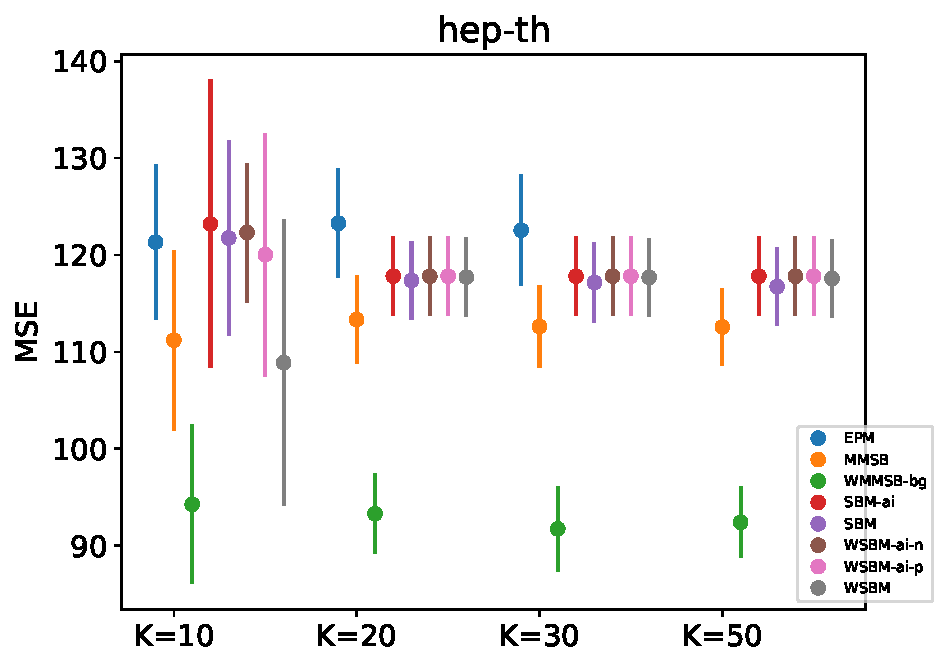
\includegraphics[width=0.23\textwidth]{fig2/hep-th_wsim3_evo2__}
\end{subfigure}  
\begin{subfigure}
         \centering
      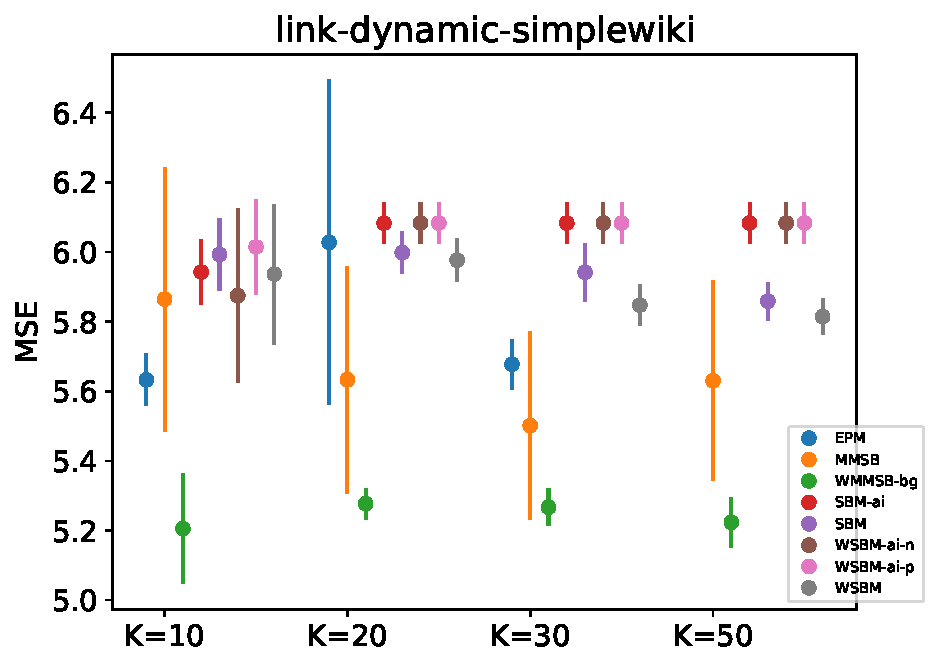
\includegraphics[width=0.23\textwidth]{fig2/wiki-link_wsim3_evo2__}
\end{subfigure} 
\begin{subfigure}
         \centering
      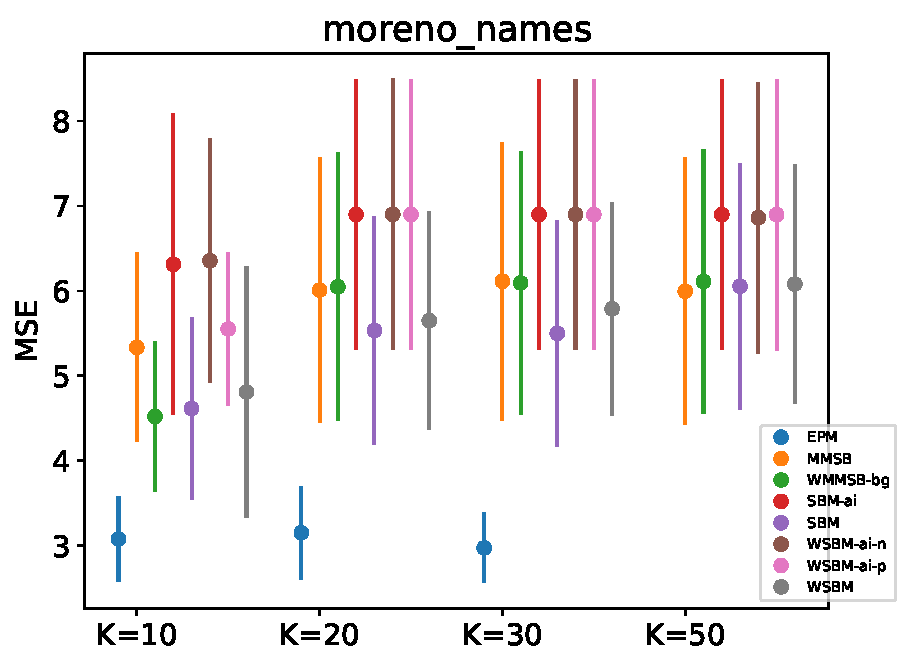
\includegraphics[width=0.23\textwidth]{fig2/moreno_names_wsim3_evo2__}
\end{subfigure} 
\begin{subfigure}
         \centering
      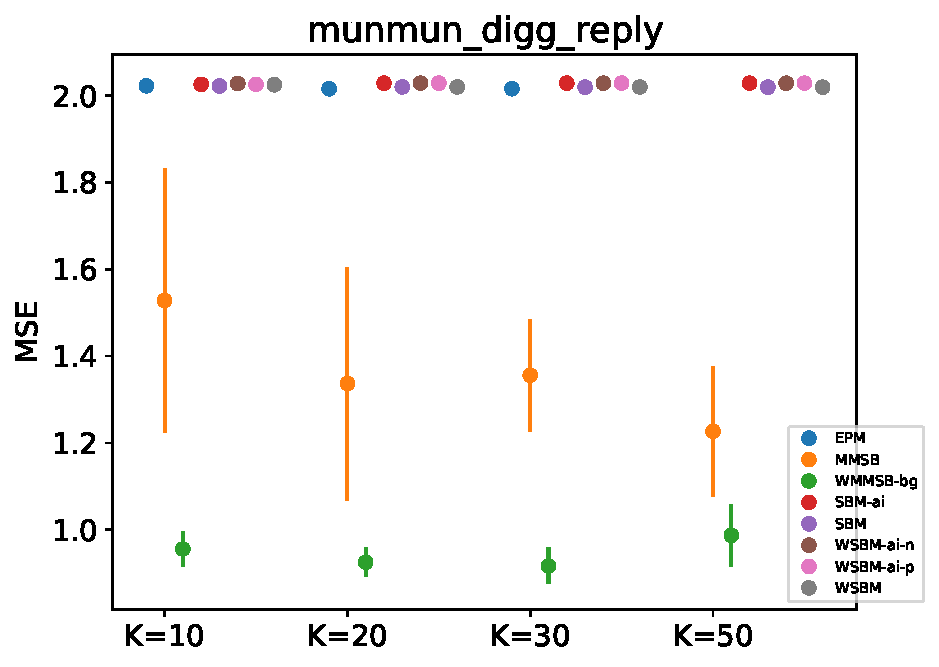
\includegraphics[width=0.23\textwidth]{fig2/digg-reply_wsim3_evo2__}
\end{subfigure} 
\begin{subfigure}
         \centering
      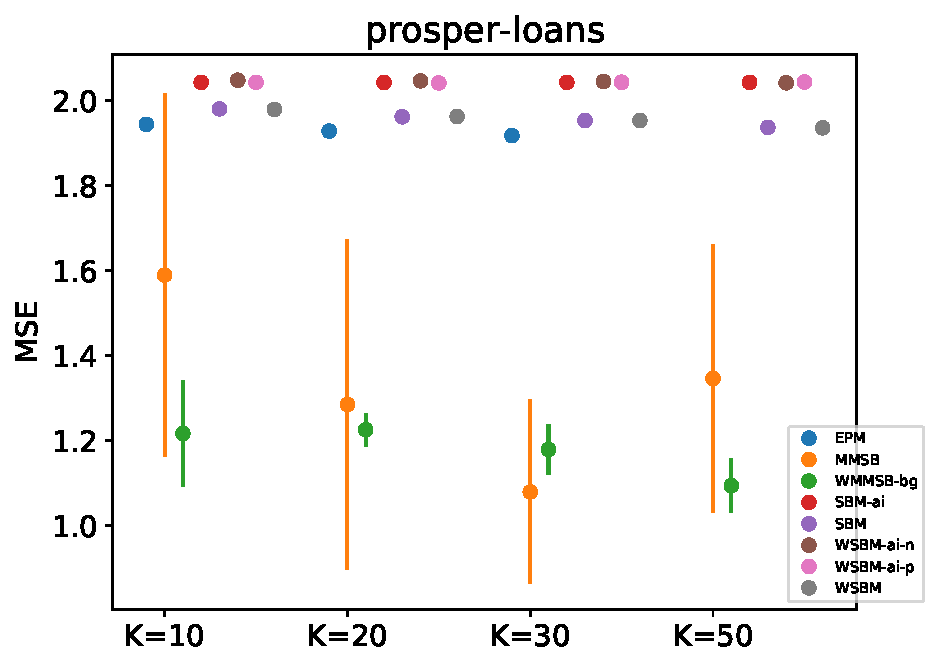
\includegraphics[width=0.23\textwidth]{fig2/prosper-loans_wsim3_evo2__}
\end{subfigure} 
\begin{subfigure}
         \centering
      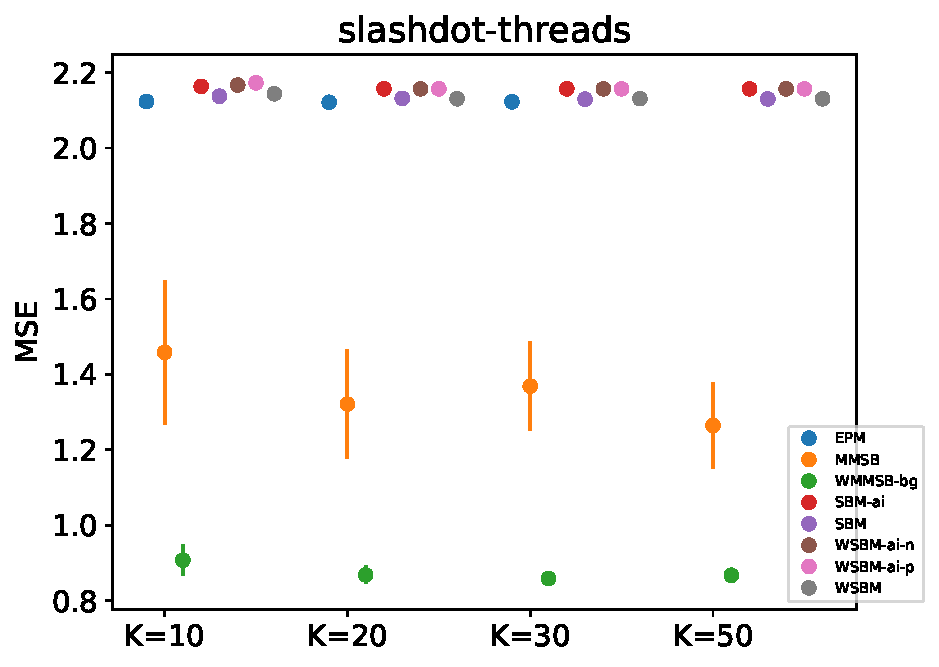
\includegraphics[width=0.23\textwidth]{fig2/slashdot_wsim3_evo2__}
\end{subfigure} 
\caption{Performance sensibility when the number of latent classes vary from $K=10$ to $K=50$.}


   \label{fig:k_evolv-app}
\end{figure}

Figure \ref{fig:k_evolv-app} displays, for six datasets, the evolution of the MSE scores when the number of latent classes, $K$, varies from 10 to 50. These results confirm the ones reported in Figure~\ref{fig:k_evolv}, Section~\ref{sec:exps} on the stability of the different models, for weight prediction, with respect to the number of latent classes.
%\section{Reproducible Research}
%
%We published our implementation within a platform that aims to ease the development of reproducible complex experiments. We are maintaining this platform that we released under open-source license.\footnote{The name of the project is anonymized.}
%
%To reproduce our results, one can proceed as follows:
%\begin{itemize}
%\item Install the XXX project:   %\lstinline|git clone https://github.com/*/XXX|  
%    \begin{lstlisting}[language=bash]
%          $ git clone https://github.com/*/*
%          $ cd XXX && make install
%    \end{lstlisting}
%\item Fit all the models on all the corpus, and save the results:
%\begin{lstlisting}[language=bash]
%        $ XXX online_roc -x fit -w --repeat 0 1 2 3 4 5 6 7 8 9 
%\end{lstlisting}
%\item Parallelization can be obtained by adding the options \lstinline|--cores NUMBER_OF_CORES|,
%\item Figures can be plotted with the command:  
%\begin{lstlisting}[language=bash]
%        $ XXX online_roc -x roc_evolution2 --repeat 0 1 2 3 4 5 6 7 8 9
%\end{lstlisting}
%\end{itemize}
%
